\chapter{Tendermint Consensus}
\label{ch:tendermint}

This chapter presents the Tendermint consensus algorithm and communicates the intuitions underlying its security.

\section{Tendermint Overview}

Tendermint is a blockchain based algorithm for the secure replication of a state
machine.
The algorithm is summarized in Figure \ref{fig:tendermint_summary}, 
its key properties as a replicated state machine are summarized in Figure \ref{fig:tendermint_guarantees}, 
and its key security properties are summarized in Figure \ref{fig:tendermint_security}.
The key data types are given in Figure \ref{fig:tendermint_types}.

\begin{figure}[]
	
\underline{Consensus State Rules}
\begin{description}
	\item[Proposal:] Wait up to \emph{TimeoutPropose} for a proposal from the correct validator for the current height and round.
	\item[Prevote:]  If a proposal comes with a valid signature from the correct proposer for a validator’s current height and round, and the validator is not locked, it should prevote for the proposal block. Else, prevote nil.
	\item[Precommit:] If a validator receives prevotes from $+\frac{2}{3}$ validators for the same block, it should precommit for that block. If the $+\frac{2}{3}$ prevotes are not for the same block, it should wait \emph{TimeoutPrevote}, and then precommit nil.
	\item[Commit:] If a validator receives precommits from $+\frac{2}{3}$ validators for the same block, it should commit that block, and go to the next height.  If the $+\frac{2}{3}$ prevotes are not for the same block, it should wait \emph{TimeoutPrecommit}, and then go to the next round.
\end{description}

\underline{Broadcast Rules}
\begin{description}
	\item[No Double Signing:] a validator only signs for each message type (proposal, prevote, precommit) once at a given height and round.
	\item[Prevote The Lock:] A validator is locked on the last block they precommitted, and must prevote for that block in future rounds at that height.
	\item[Unlock On Polka:] a validator may only unlock if there have been $+\frac{2}{3}$ prevotes at a round after they locked. 
\end{description}
Violation of any of the Broadcast Rules is detectable and should be punished.

\caption[Summary of Tendermint protocol rules]{Summary of rules in the tendermint protocol. 
$+\frac{2}{3}$ validators is short for ``more than two-thirds of validators''}

	\label{fig:tendermint_summary}
\end{figure}

\begin{figure}[]
	\textbf{Tendermint Safety Guarantees}
\begin{description}
  \item[Proposer Safety] \hfill \\
	There is at most one valid proposer for every term.
  \item[Validator Append Only] \hfill \\
	A validator never overwrites or deletes blocks it has committed.
  \item[Proposer Completeness] \hfill \\
	If a block is committed at a given height, then that block will be present in the chain of all proposers at greater heights.
  \item[State Machine Safety] \hfill \\
	If a validator has applied a block at a given height to its state machine, no other validator will ever apply a different block for the same height.
\end{description}
\caption[Tendermint Safety Guarantees]{Tendermint guarantees that all of these properties are true, at all times, within the security guarantee. This set of properties was taken practically verbatim from \cite{raft_thesis}.}

	\label{fig:tendermint_guarantees}
\end{figure}

\begin{figure}[]
	
\textbf{Tendermint Security Guarantees}
\begin{description}
  \item[Byzantine Fault Tolerance] \hfill \\
	All properties in \ref{fig:tendermint_guarantees} are satisfied so long as fewer than one-third of validators are Byzantine.
  \item[Deterministic Accountability] \hfill \\
	If one-third or more of validators, but less than half, are Byzantine, and thereby compromise safety, 
	they can be specifically identified and held accountable to their actions.
\end{description}
\caption[Tendermint Security Guarantees]{Tendermint guarantees these security properties, making it more suitable than algorithms like Raft and Paxos, and even other BFT algorithms like PBFT, for consortia with potentially malicious or untrusted actors}

	\label{fig:tendermint_security}
\end{figure}

\lstset{xleftmargin=-1in}
\floatstyle{plain}
\restylefloat{figure}
\begin{figure}[]
	
\vspace*{-1.5in}

\begin{lstlisting}

// Proposal for a block at a given height and round, signed by the proposer
type Proposal struct {
  Height           int                     
  Round            int                     
  BlockHash        []byte                  
  Signature        crypto.SignatureEd25519  // 64 bytes
}

// Represents a prevote or precommit vote from validators for consensus.
type Vote struct {
  Height           int                     
  Round            int                     
  Type             byte                     // 1 for prevote, 2 for precommit
  BlockHash        []byte                   // empty if vote is nil
  Signature        crypto.SignatureEd25519  // 64 bytes
}

// A vote message, gossiped to peers
type VoteMessage struct {
  ValidatorIndex int
  Vote           *types.Vote
}

// A proposal message, gossiped to peers
type ProposalMessage struct {
  Proposal *types.Proposal
}

// Current local state of a validator's consensus machine
type RoundState struct {
  Height             int // Height we are working on
  Round              int
  Step               RoundStepType
  CommitTime         time.Time // Subjective time we received +2/3 precommits 
  Validators         *types.ValidatorSet
  Proposal           *types.Proposal
  ProposalBlock      *types.Block
  LockedRound        int
  LockedBlock        *types.Block
  Votes              *HeightVoteSet // Votes from all rounds at this height
  CommitRound        int            //
  LastCommit         *types.VoteSet // Last precommits at Height-1
  LastValidators     *types.ValidatorSet
}
\end{lstlisting}

\caption[Summary of Tendermint protocol data types]{Summary of data types in the Tendermint protocol}

	\label{fig:tendermint_types}
\end{figure}
\floatstyle{boxed}
\restylefloat{figure}

Tendermint begins with a set of \emph{validators}, each of which is responsible for maintaining a full copy of the replicated state,
and for participating by proposing new blocks (batches of transactions), and voting on them.
Each block is assigned an incrementing index, or \emph{height}, 
such that a valid blockchain has only one valid block at each height.
At each height, validators take turns proposing new blocks in \emph{rounds}, 
such that for any given round there is at most one valid proposer.
It may take multiple rounds to commit a block at a given height due to the asynchrony of the network,
and the network may halt altogether if more than one-third of the validators are offline or partitioned.
Validators engage in two phases of voting on a proposed block before it is committed, 
and follow a simple locking mechanism which prevents any coalition of up to one third malicious validators from compromising safety.

Note that the core round-based voting mechanism is the consensus algorithm, 
which is strung together into blocks to yield atomic broadcast.
Each block contains some metadata, known as its \emph{header}, 
which includes the hash of the block at the previous height, resulting in a hash chain.
The header also includes the block height, local time the block was proposed, 
and the Merkle root hash of transactions included in the block.

The consensus algorithm can be roughly divided into the following, somewhat orthogonal, components:

\begin{itemize}

\item{Proposals: a new block must be proposed by the correct proposer at each round, and gossiped to the other validators. If a proposal is not received in sufficient time, the proposer should be skipped.}

\item{Votes: two phases of voting must occur to ensure optimal Byzantine fault tolerance. They are called \emph{pre-vote} and \emph{pre-commit}. A set of pre-commits from more than two-thirds of the validators for the same block at the same round is a \emph{commit}.}

\item{Locks: Tendermint ensures that no two validators commit a different block at the same height, presuming less than one-third of the validators are malicious. This is achieved using a locking mechanism which determines how a validator may pre-vote or pre-commit depending on previous pre-votes and pre-commits at the same height. Note that this locking mechanism must be carefully designed so as to not compromise liveness.}

\end{itemize}

As will be seen, Tendermint affords an ability to identify and hold accountable malicious validators, thus providing greater security guarantees than competing algorithms in the event that one-third or more Byzantine validators compromise safety.

\section{Blockchain}

Tendermint operates on batches (blocks) of transactions at a time.
Continuity is maintained from one block to the next by explicitly linking each block to the one before it 
via it's cryptographic hash, forming a blockchain. 
The blockchain contains the ordered transaction log and evidence that the block was committed 
by the validators.

\subsection{Why Blocks?}
Consensus algorithms typically commit transactions one at a time by design, 
and implement batching after the fact.
As mentioned in Chapter \ref{ch:background}, 
tackling the problem from the perspective of batched atomic broadcast
results in two primary optimizations, which give us more throughput and fault-tolerance:

\begin{itemize}
\item{Bandwidth optimization: since every commit requires two rounds of communication across all validators, 
	batching transactions in blocks amortizes the cost of a commit over all the transactions in the block.}
\item{Integrity optimization: the hash chain of blocks forms an immutable data structure, much like a Git repository, enabling authenticity checks for sub-states at any point in the history.}
\end{itemize}

Blocks induce another effect as well, which is more subtle but potentially important. 
They increase the minimum latency of a transaction to that of the whole block, 
which for Tendermint is on the order of hundreds of milliseconds to seconds.
Traditional serializable database systems provide commit latencies on the 
order of milliseconds to tens of milliseconds.
They are able to do this because they are not Byzantine Fault Tolerant, 
requiring only one round of communication (instead of two)
and responses from over half of the replicas (instead of two-thirds).
However, unlike the fast commit times interrupted by leader elections in other algorithms,
Tendermint provides a more regular pulse that is more responsive to the overall health of the network, 
in terms of node failures and asynchrony.

What role such pulses might play in the coherence of 
communicating autonomous systems on the internet is yet to be determined,
though purposefully induced latency has shown promise in the financial markets \cite{iex}.

\subsection{Block Structure}

The purpose of blocks is to contain a batch of transactions, and to link to the previous block.
The link comes in two forms: the previous block hash,
and the set of pre-commits which caused the previous block to be committed, also known as the $LastCommit$.
Thus a block is composed of three parts: the block header, the list of transactions, and the $LastCommit$.
The composition of the header is given in Figure \ref{fig:header}

\begin{figure}[]
	
\begin{verbatim}
type Header struct {
	ChainID            string        
	Height             int           
	Time               time.Time     
	NumTxs             int           
	LastBlockHash      []byte        
	LastBlockParts     PartSetHeader 
	LastCommitHash []byte       // Merkle root hash of LastCommit
	DataHash           []byte   // Merkle root hash of transaction 
	ValidatorsHash     []byte   // Merkle root hash of validator set
	AppHash            []byte   // state Merkle root from previous block's transactions
}

type PartSetHeader struct {
	Total int    
	Hash  []byte 
}
\end{verbatim}
	\caption[Block Header Structure]{The fields required for a valid block header. The validity of all fields is checked before pre-commit}

	\label{fig:header}
\end{figure}

\section{Tendermint Basics}

In order to provide tolerance to a single Byzantine fault, a Tendermint network must contain at minimum four validators.
Each validator must possess an asymmetric cryptographic key-pair for producing digital signatures.
Validators start from a common \emph{genesis} state, which contains the initial list of validators in terms of their public keys.
All proposals and votes must be signed by the respective validator's private key, and can hence be verified by every other validator.
It is helpful to assume that up to one-third of validators are malicious, co-operating in arbitrary ways to subvert system safety or liveness.

Consensus begins for block 1, round 0; the proposer is the first validator listed in the genesis.
The outcome of a round is either a commit, or a decision to move to the next round.
With a new round comes the next proposer.
Using multiple rounds gives validators multiple opportunities to come to consensus in the event of network asynchrony or validator failures.

In contrast to algorithms which require a form of leader election, Tendermint has a new leader (the proposer) for each round.
Validators vote to skip to the next round in the same way they vote to accept the proposal,
lending the protocol a uniformity of mechanism that is absent from algorithms with an explicit leader-election program.

The beginning of each round has a weak dependence on synchrony as it utilizes local clocks to determine when to skip a proposer.
That is, if a validator does not receive a proposal within a locally measured \emph{TimeoutPropose} of entering a new round, it can vote to skip the proposer.
Inherent in this mechanism is the assumption that, at least eventually, the proposal will be delivered within \emph{TimeoutPropose}, which may itself increment with each round.
This assumption is discussed more fully in Chapter \ref{ch:related}.

After the proposal, rounds proceed in a fully asynchronous manner - a validator makes progress only after hearing from more than two-thirds of the other validators.
This relieves any sort of dependence on synchronized clocks or bounded network delays,
but implies that the network will halt if one-third or more of the nodes become unresponsive.
This circuit of weakly synchronous proposals, followed by asynchronous voting, 
is depicted in Figure \ref{fig:consensus_logic}.

\begin{figure}[]
	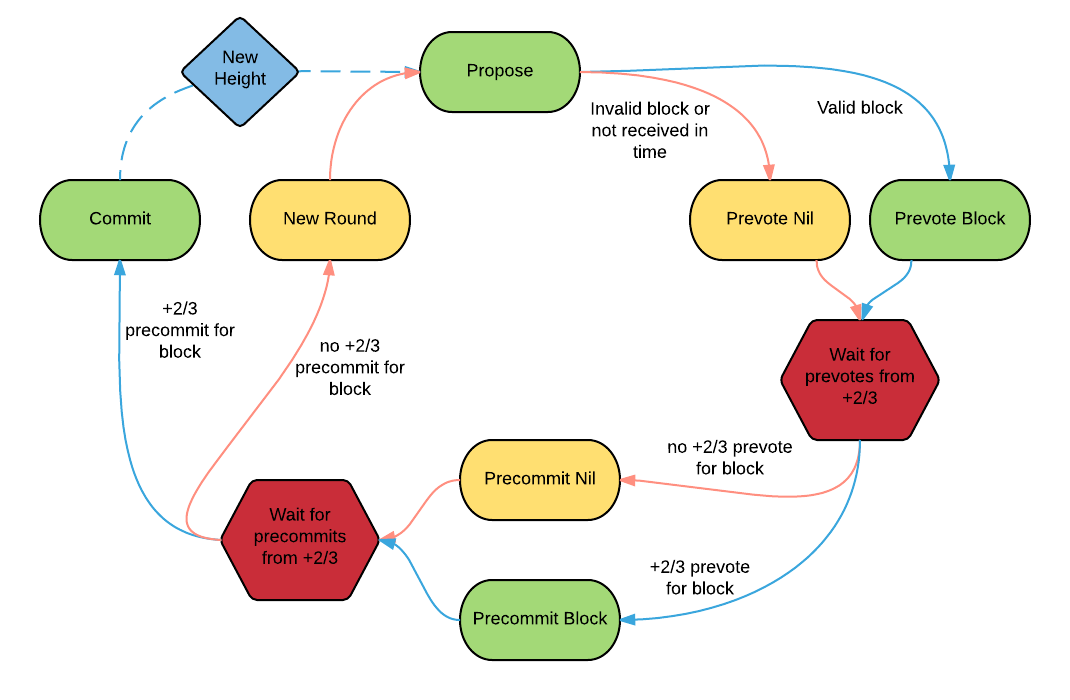
\includegraphics[width=\linewidth,height=\textheight,keepaspectratio]{figures/diagrams/consensus_logic.png}
    	\centering
	\caption[Overview of Tendermint consensus logic]{
After the proposal step, validators only make progress after hearing from two-thirds or more (+2/3) of other validators.}
	\label{fig:consensus_logic}
\end{figure}

To round-skip safely, a small number of \emph{locking} rules are introduced which force validators to justify their votes.
While we don't necessarily require them to broadcast their justifications in real time, we do expect them to keep the data,
such that it can be brought forth as evidence in the event that safety is compromised by sufficient Byzantine failures.
This accountability mechanism enables Tendermint to provide stronger guarantees in the face of such failure than eg.~PBFT,
which provides no guarantees if a third or more of the validators are Byzantine.

Validators communicate using a diverse set of messages for managing the blockchain, application state, peer network, and consensus.
The core consensus algorithm, however, consists of just two messages:

\begin{itemize}
\item{\emph{ProposalMsg}: a proposal for a block at a given height and round, signed by the proposer.}
\item{\emph{VoteMsg}: a signed vote for a proposal.}
\end{itemize}

In practice, we use additional messages to optimize the gossiping of block data and votes, as discussed in Chapter \ref{ch:subprotocols}.

\section{Proposals}

Each round begins with a proposal. 
The propser for the given round takes a batch of recently received transactions from its local cache (the Mempool, see Chapter \ref{ch:subprotocols}),
composes a block, and broadcasts a signed ProposalMsg containing the block.
If the proposer is Byzantine, it might broadcast different proposals to different validators.

Proposers are ordered via a simple, deterministic round robin, 
so only a single proposer is valid for a given round, 
and every validator knows the correct proposer. 
If a proposal is received for a lower round, or from an incorrect proposer, it is rejected.

Cycling of proposers is necessary for Byzantine tolerance. 
For instance, in Raft, if an elected leader is Byzantine and maintains strong network connections to other nodes,
it can completely compromise the system, destroying all safety and liveness guarantees.
Tendermint preserves safety via the voting and locking mechanisms, 
and maintains liveness by cycling proposers, so if one won't process any transactions, others can pick up.
Perhaps more interestingly, validators can vote through governance modules (see Chapter \ref{ch:governance}) to remove or replace Byzantine validators.

\section{Votes}

Once a complete proposal is received by a validator, 
it signs a pre-vote for that proposal and broadcasts it to the network.
If a validator does not receive a correct proposal within \emph{ProposalTimeout}, 
it signs and broadcasts a \emph{nil-pre-vote} instead.

In Byzantine environments, a single stage of voting,
where each validator casts only one vote,
is not sufficient to ensure safety.
This can be seen via a proof by contradiction.
Suppose that a single round of voting, where more than two-thirds vote for a single block, were sufficient to commit the block.
Consider a network with validators Val1, Val2, Val3, and Val4, where Val1 is Byzantine.
Suppose Val1 both votes for the proposal, and nil-votes (it is Byzantine).
Suppose Val2 and Val3 vote, while Val4 nil-votes (it didn't receive the proposal in time).
Now, suppose Val2 sees the pre-votes from Val1, itself, and Val3, and hence commits the proposed block,
but Val3 and Val4 only see messages from each other and the nil-prevote from Val1.
Now Val3 and Val4 go to the next round, while Val2 has already committed, and only Val1 is Byzantine.
Val1 also goes to the next round and the three of them commit a block.
Now Val2 has committed one block while Val3 and Val4 have committed another while less than one-third of the validators (only Val1) are Byzantine,
thus violating safety. 

The importance of the example is to illustrate why using only a single round of voting
is not sufficient if some validators can be Byzantine.
A single round of voting allows validators to tell each other what they know about the proposal.	
But to tolerate Byzantine faults (which amounts, essentially to lies, fraud, deceipt, etc.), 
they must also tell each other what they know about what other validators have professed to know about the proposal.

Thus, pre-voting is a preparation phase, in which validators synthesize what other validators know.
A pre-vote for a block is a vote to prepare the network to commit the block.
A nil-pre-vote is a vote to prepare the network to move to the next round.
In an ideal round with an online proposer, more than two-thirds of validators will pre-vote for the proposal.
A set of more than two-thirds of pre-votes for a single block at a given round is known as a \emph{polka}\footnote{The original term used was PoL, or PoLC, for Proof-of-Lock or Proof-of-Lock-Change. The term evolved to polka as it was realized the validators are doing the polka.}.
A set of more than two-thirds of pre-votes for nil is a \emph{nil-polka}

When a validator receives a polka (read: more than two-thirds pre-votes for a single block), 
it has received a signal that the network is prepared to commit the block,
and serves as justification for the validator to sign and broadcast a pre-commit vote for that block.
Sometimes, due to network asynchrony, a validator may not receive a polka, or there may not have been one. 
In that case, the validator is not justified in signing a pre-commit for that block, 
and must therefore sign and publish a pre-commit vote for nil (nil-pre-commit).
That is, it is considered malicious behaviour to sign a pre-commit without justification from a polka.

A pre-commit is a vote to actually commit a block.
A nil-pre-commit is a vote to actually move to the next round.
If a validator receives more than two-thirds pre-commits for a single block, 
it commits that block, computes the resulting state,
and moves on to round 0 at the next height.
If a validator receives more than two-thirds nil-pre-commits,
it moves on to the next round.

\section{Locks}

Ensuring safety across rounds can be tricky, 
as circumstances must be avoided which would provide justification for two different blocks to be committed at two different rounds at the same height.
In Tendermint, this problem is solved via a \emph{locking} mechanism.
In essence, once a pre-commit is cast, a validator is \emph{locked} on the associated block, and must follow certain locking rules.
There are two rules of locking:

\begin{itemize}
\item{Prevote-the-Lock: a validator must pre-vote for the block they are locked on. 
	This prevents validators from pre-committing one block in one round, 
	and then contributing to a polka for a different block in the next round, 
	thereby compromising safety.}
\item{Release-Lock-on-Polka: a validator may only release a lock after seeing a polka or nil-polka at a round greater than that at which it locked.
	This allows validators to unlock if they pre-committed something the rest of the network doesn't want to commit,
	thereby protecting liveness, but does it in a way that does not compromise safety,
	by only allowing unlocking if there has been a polka in a round after that in which the validator became locked.}
\end{itemize}


For simplicity, a validator is considered to have locked on nil at round -1 at each height, so that Release-Lock-on-Polka implies that a validator cannot precommit at all at a new height until they see a polka.

These rules can be understood more intuitively by way of examples. 
Consider again our four validators, and suppose there is a proposal for $blockA$ at round $R$. 
Suppose there is a polka for $blockA$, but Val1 doesn't see it, and precommits nil, while the others precommit for $blockA$.
Now suppose the only one to see all precommits is Val4, while the others, say, don't see Val4's precommit (they only see their two precommits and Val1's nil-precommit).
Val4 will now commit the block, while the others go to round $R+1$.
Since any of the validators might be the new proposer, if they can propose and vote for any new block, say $blockB$, then they might commit it and compromise safety, since Val4 already committed $blockA$.
Note that there isn't even any Byzantine behaviour here, just asynchrony!

Locking solves the problem by forcing validators to stick with the block they pre-committed, since other validators might have committed based on those precommits (as Val4 did in this example).
In essence, once more than two-thirds precommit a block in a round, the network is locked on that block,
which is to say it must be impossible to produce a valid polka for a different block at a higher round.
This is direct motivation for Prevote-the-Lock.

Prevote-the-Lock is not sufficient, however. There must be a way to unlock, lest we sacrifice liveness.
Consider a round where Val1 and Val2 precommitted $blockA$ while Val3 and Val4 precommitted nil.
They all move to the next round, and $blockB$ is proposed, which Val3 and Val4 prevote for.
Suppose Val1 is Byzantine, and prevotes for $blockB$ as well (despite being locked on $blockA$), resulting in a polka.
Suppose Val2 does not see the polka and precommits nil, while Val1 goes off-line and Val3 and Val4 precommit $blockB$. 
They move to the next round, but Val2 is still locked on $blockA$, while Val3 and Val4 are now locked on $blockB$, 
and since Val1 is offline, they can never get a polka. Hence, we've compromised liveness with less than a third (here, only one) Byzantine validators.

The obvious justification for unlocking is a polka. Once Val2 sees the polka for $blockB$ (which Val3 and Val4 used to jusitfy their precommits for $blockB$), 
it ought to be able to unlock, and hence precommit $blockB$.
This is the motivation for Release-Lock-on-Polka, which allows validators to unlock (and precommit a new block) if they have seen a polka in a round greater than that in which they locked.

A complete description of Tendermint consensus is given in Figure \ref{fig:tendermint_consensus_protocol}.

\section{Safety}

Here we sketch a brief proof of Tendermint's safety guarantee, namely, 
the State Machine Safety property, that for two validators to apply different blocks at the same height
requires at least one-third of valdiators to be Byzantine.

Referring back to the safety guarantees in Figure \ref{fig:tendermint_guarantees}, 
note that Proposer Safety, Validator Append Only, and Proposer Completeness are trivially satisfied by the protocol, 
in particular through the use of a round-robin for the proposer selection and hash links to connect blocks,
and by not allowing blocks to be overwritten.

Suppose that two blocks are committed at the same height.
Let the blocks be $blockA$ and $blockB$, and let them be committed in rounds $R_A$ and $R_B$, respectively, with $R_A < R_B$.
Since each commit requires more than two-thirds of validators, 
two commits requires that more than a third of validators sign for both commits.
Let this set of validators be $D$.
Note that if $R_A = R_B$, a single proposer must have proposed two blocks at the same round, 
and the validators in $D$ must have precommitted for both $blockA$ and $blockB$ in that same round, 
making the proof trivial, since double signing within a round is Byzantine.

With blocks committed in different rounds, however, 
we must show that at least a third of validators violated the locking rules.
We already know that the validators from $D$ lock on $blockA$ in $R_A$.
To unlock from $blockA$, and precommit for $blockB$, 
they must observe a polka for $blockB$ at round $R_P$, where $R_A < R_P <= R_B$.
A polka requires more than two-thirds of validators to prevote for the same block.
Since more than two-thirds locked on $blockA$ at round $R_A$, 
a polka for a different block at a higher round requires more than a third to violate Prevote-the-Lock.
Given Proposer Safety, Validator Append Only, and Proposer Completenes,
this guarantees State Machine Safety assuming less than one-third of validators are Byzantine.

In future work, we aim to provide a more formal proof of Tendermint's correctness 
and the ability to identify validators which violated locking rules.


%
%- Proposer Safety condition implied by protocol
%- Validator Append Only condition implied by the protocol
%- Proposer Completeness guaranteed by the merkle hash chain
%
%Need to show Block Matching, State Machine Safety, and Deterministic Accountability.
%Locking rules give us lemmas about polkas.
%


\section{Faults and Availability}

As a BFT consensus algorithm, Tendermint can tolerate Byzantine failure in up to (but not including) one-third of validators.
This means nodes can crash, send different and contradictory messages to different peers, refuse to relay messages, or otherwise behave arbitrarily,
without compromising safety or liveness (with the usual FLP caveat for liveness).

There are two places in the protocol where we can make optimizations for asynchrony by utilizing timeouts based on local clocks:
after receiving two-thirds or more pre-votes, but not for a single block or nil, and after receiving two-thirds or more pre-commits, 
but not for a single block or nil.
In each case, we can sleep for some amount of time to give slower or delayed votes a chance to be received,
thereby reducing the likelihood of going to a new round without committing a block.
Clocks do not need to be synced across validators, as they are reset each time a validator observes votes from two-thirds or more others.

If a third or more of validators crash, the network halts, 
as no validator is able to make progress without hearing from more than two-thirds of the validator set.
The network remains available for reads, but no new commits can be made.
As soon as validators come back on-line, they can carry on from where they left in a round. 
The consensus state-machine should employ a write-ahead log,
such that a recovered validator can quickly return to the step it was in when it crashed.

If a third or more of validators are Byzantine, they can compromise safety a number of ways, 
for instance, by proposing two blocks for the same round, and voting both of them through to commit, 
or by pre-committing on two different blocks at the same height but in different rounds by violating the rules on locking.
In each case, there is clear, identifiable evidence that certain validators misbehaved. 
In the first instance, they signed two proposals at the same round, a clear violation of the rules.
In the second, they may have pre-voted for a different block in round $R$ than they locked on in $R-1$, 
a violation of the Prevote-the-Lock rule.

When using economic and governance components to incentivize and manage the consensus (Chapter  \ref{ch:governance})
these additional accountability guarantees become critical.

\section{Conclusion}

Tendermint is a weakly synchronous, Byzantine fault tolerant, state machine replication protocol,
with optimal Byzantine fault tolerance and additional accountability guarantees in the event
the BFT assumptions are violated. 
The protocol uses a round-robin approach for proposers, and uses the same mechanism to skip a proposer as to commit a proposed block.
Safety is maintained across rounds via a simple locking mechanism.

The presentation of the protocol in this chapter left out many important details, 
such as the efficient gossiping of blocks, buffering transactions, changes to the validator set, 
and the interface with application logic. These important topics are taken up in subsequent chapters.


